\section{Overall description}
Here you can see how to include an image in your document.

\begin{sidewaysfigure}
\centering
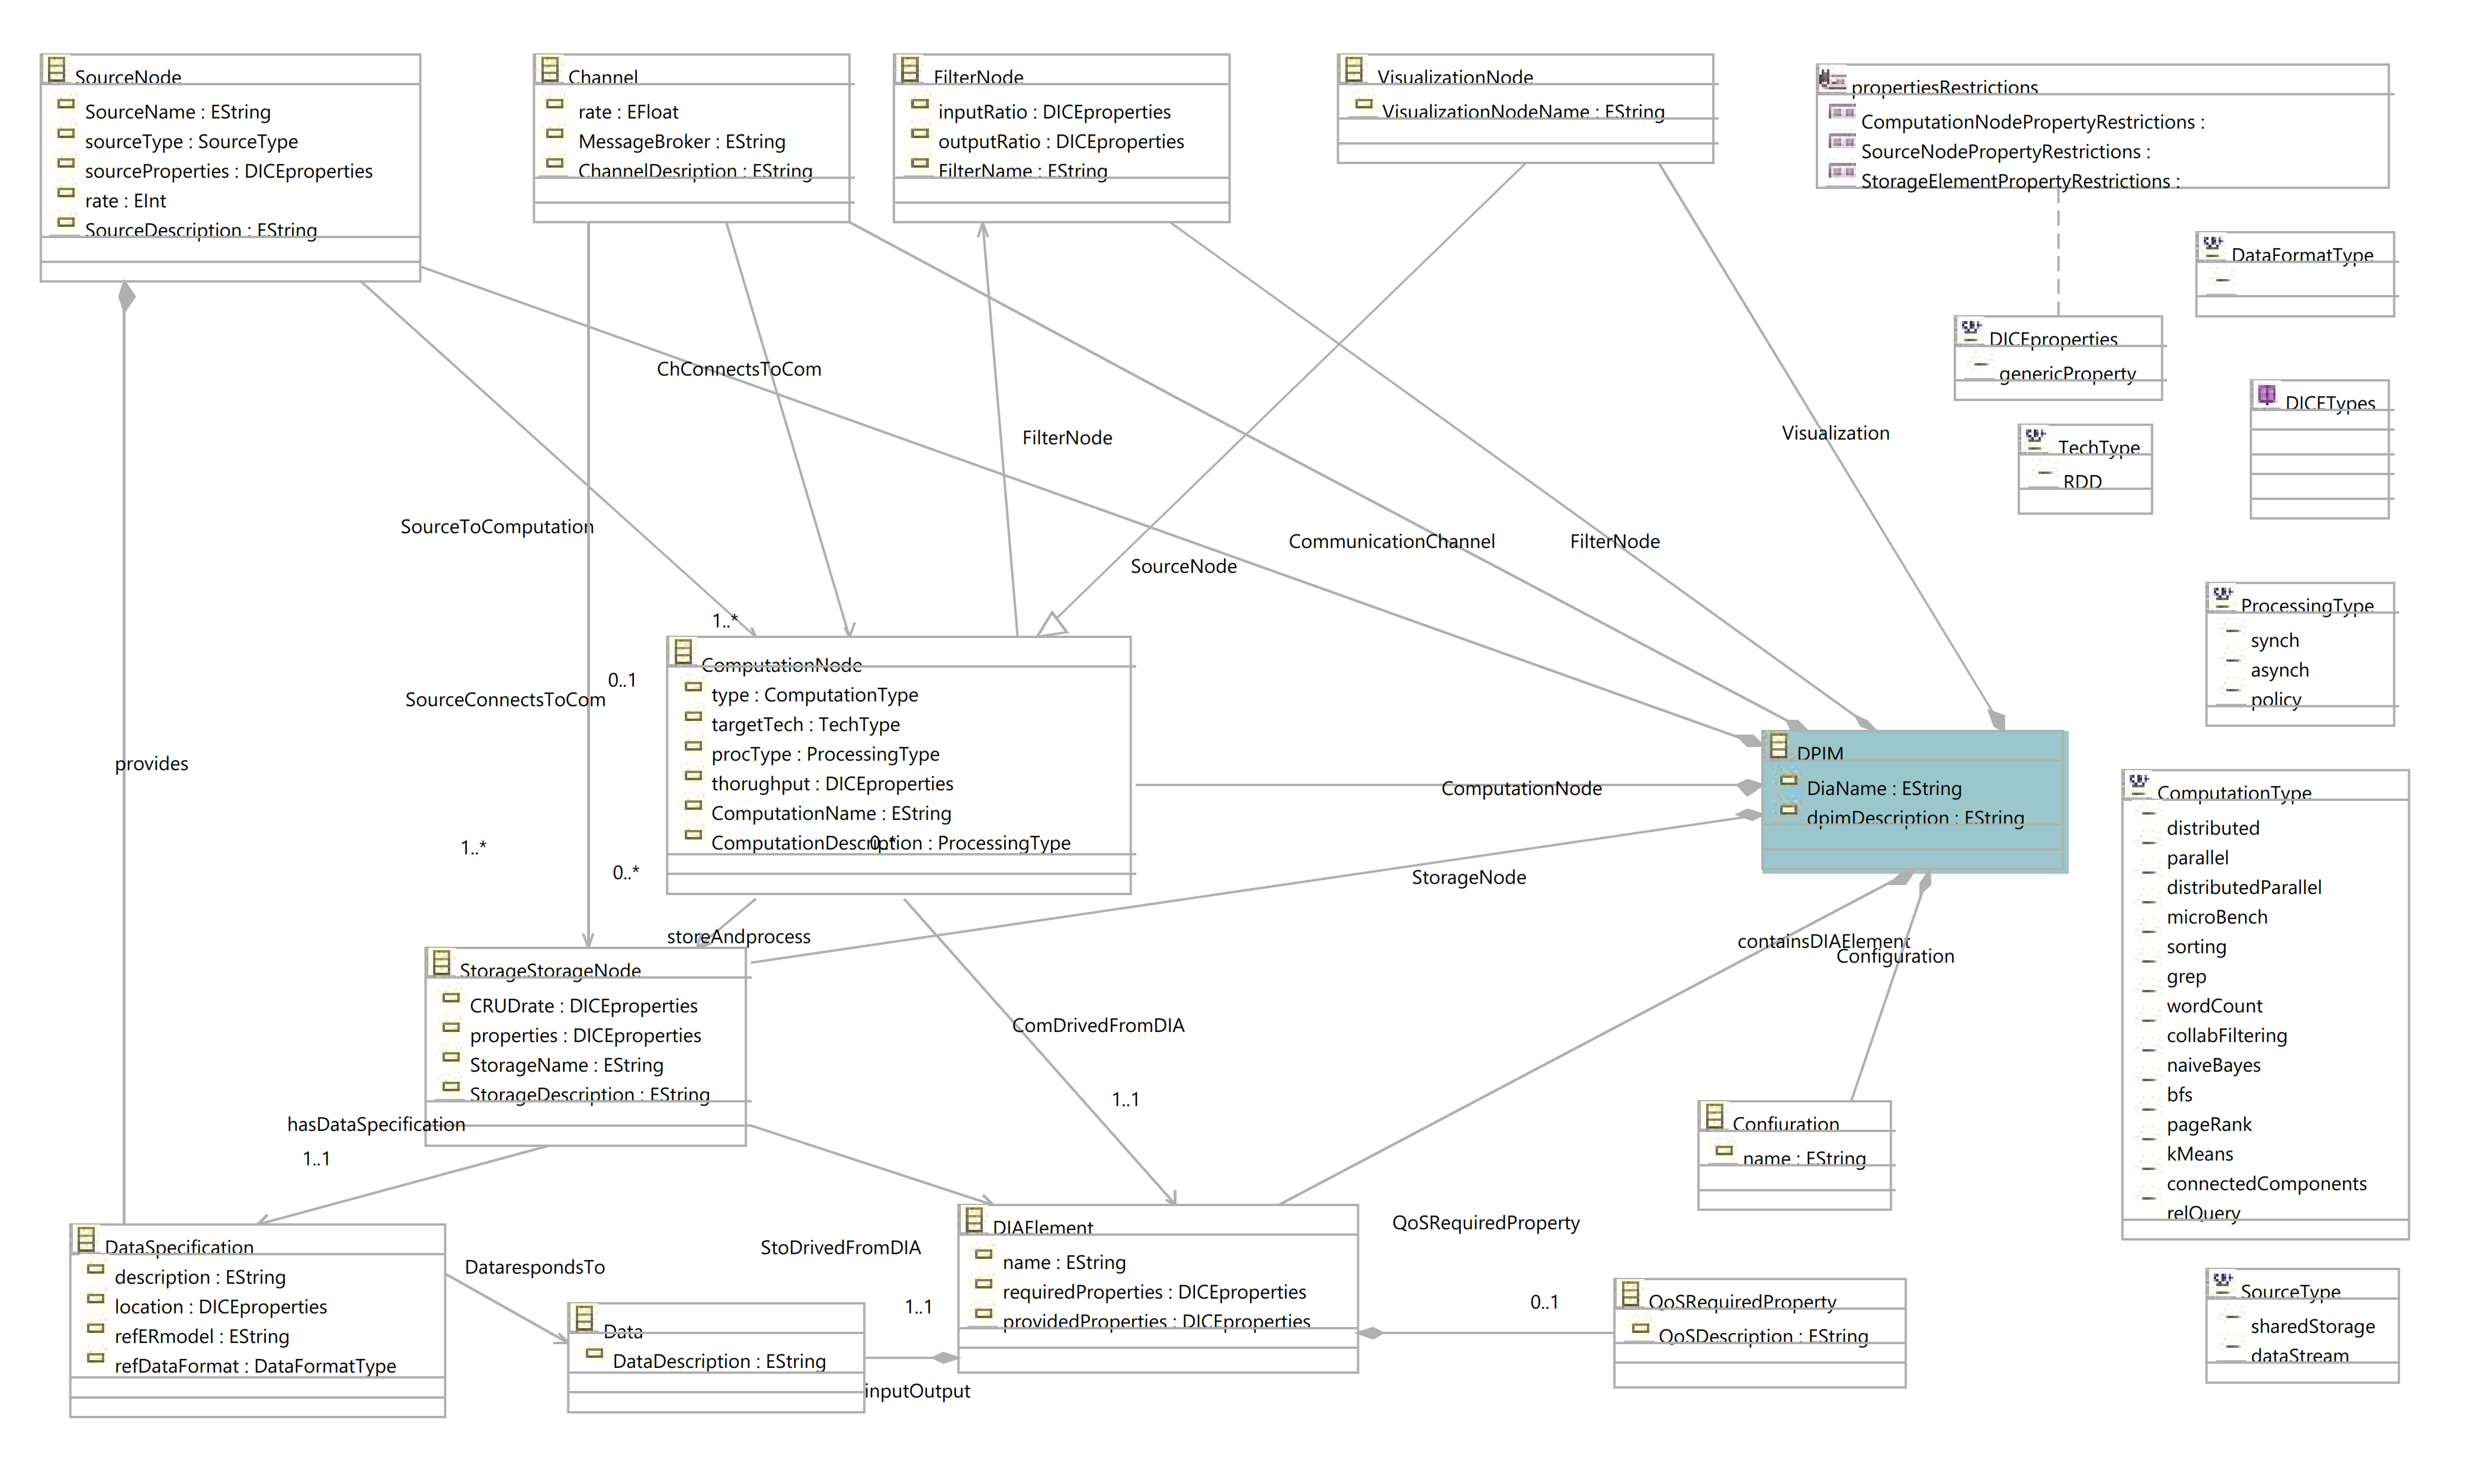
\includegraphics[width=\textwidth]{Images/11.png}
\caption{\label{fig:metamodel}DICE DPIM metamodel.}
\end{sidewaysfigure}

\begin{figure}
\centering
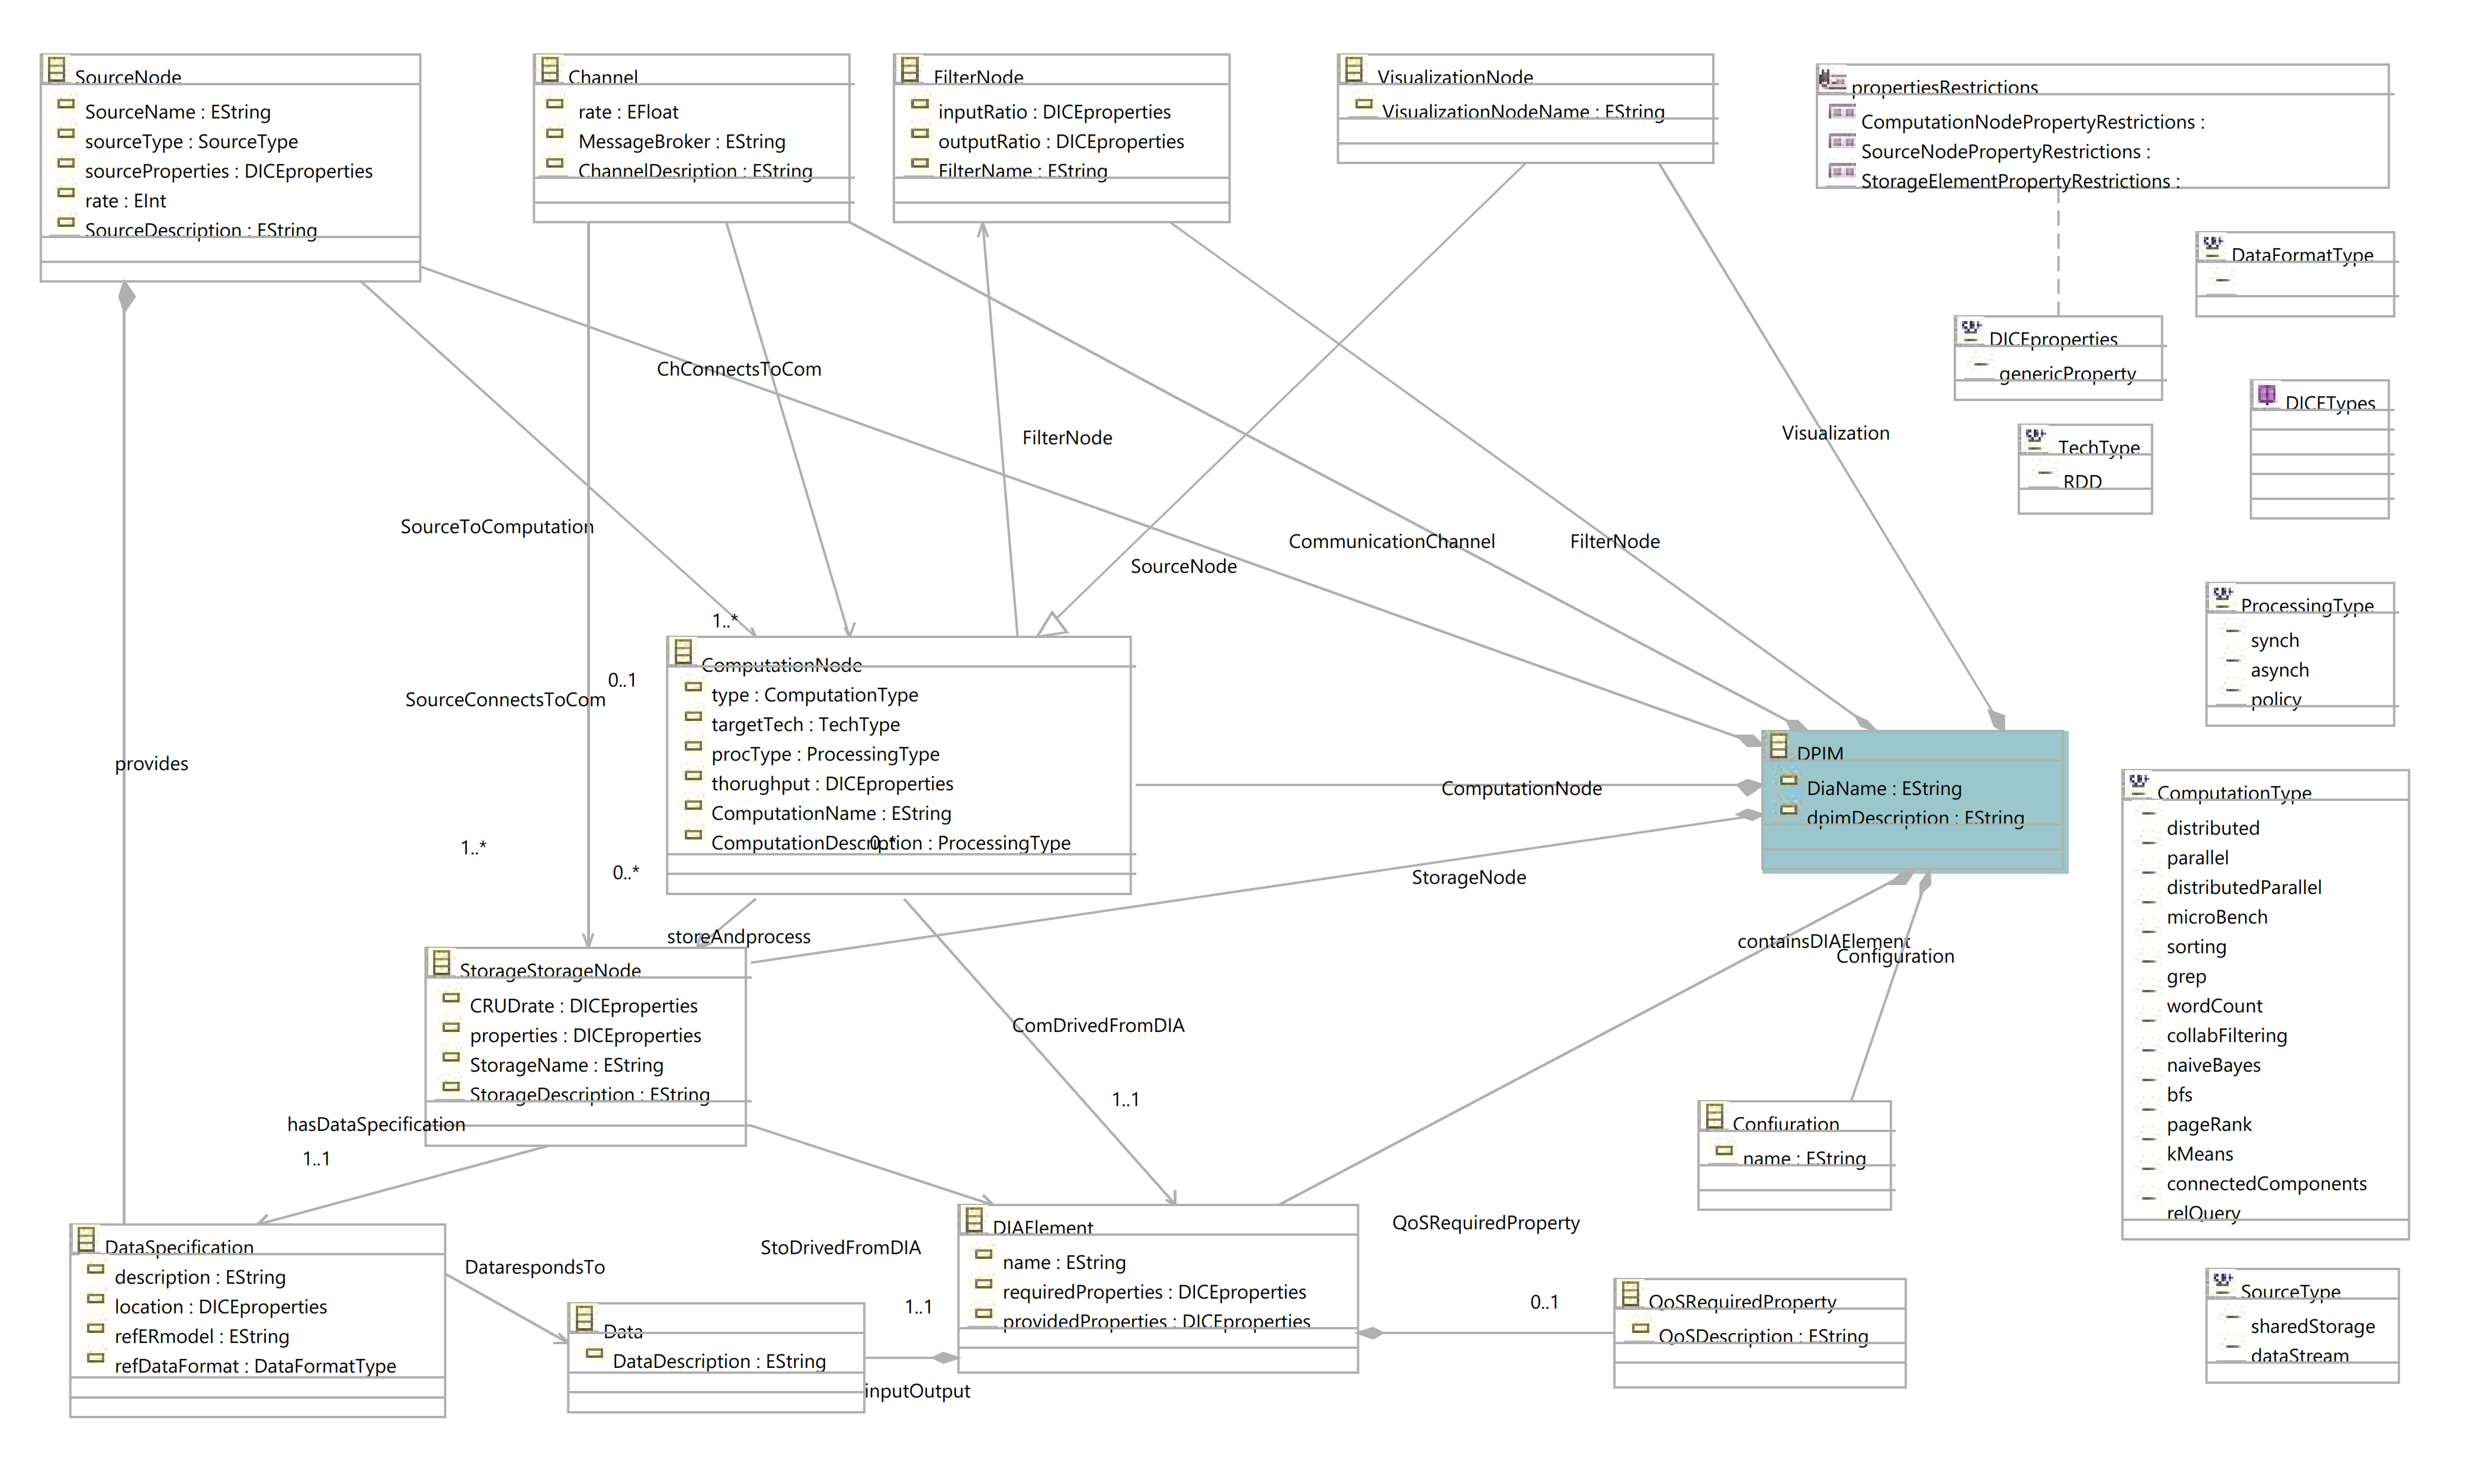
\includegraphics[width=\textwidth]{Images/11.png}
\caption{\label{fig:metamodel2}DICE DPIM metamodel in portrait form.}
\end{figure}

Here is the command to refer to another element (section, figure, table, ...) in the document: \emph{As discussed in Section~\ref{sect:overview} and as shown in Figure~\ref{fig:metamodel}, ...}. Here is how to introduce a bibliographic citation~\cite{DAM}. Bibliographic references should be included in a \texttt{.bib} file. 

Table generation is a bit complicated in Latex. You will soon become proficient, but to start you can rely on tools or external services. See for instance this \href{https://www.tablesgenerator.com}{https://www.tablesgenerator.com}. 

\subsection{Product perspective}
\subsubsection{scenarios}
\subsubsection{further details on shared phenomena}
\subsubsection{domain model: class diagrams and statecharts}
\subsection{Product functions}
most important requirements
\subsection{User characteristics}
\subsubsection{Actors}
\begin(itemize)
\item Customer: a person who grocery shops.
\item Unregistered user: a customer using CLup without being registered. They can join the virtual queue and ask/receive updates.
\item Registered user/User: a customer using Clup and who is registered on the system. They can join the virtual queue, book a shopping session and ask/receive updates.
\item Shop manager: a person who register their shop on Clup. A shop manager can register multiple shop on the system.
\item Shop: a grocery shop registered on the system. It updates periodically the people present in the store and sends updates to the manager.
\end(itemize)

\subsection{Assumptions, dependencies and constraints}
\subsubsection{Domain Assumptions}

